\documentclass[tikz,border=2pt]{standalone}
\usepackage{amsmath}
\usepackage{amssymb}
\usepackage{pgfplots}
\pgfplotsset{compat=1.18}
\usetikzlibrary{arrows.meta}
\begin{document}
% CONWIP line of five single-server exponential stations, E[S]=(2,1.5,1,0.75,0.5) hours, n cards.
% Left: MVA throughput TH_1(n) with the bounds n/5.75 (raw processing time 5.75) and 1/2 (bottleneck).
% Right: mean cycle time E[J(n)]=n/TH_1(n) with the bounds 5.75 and 2n.
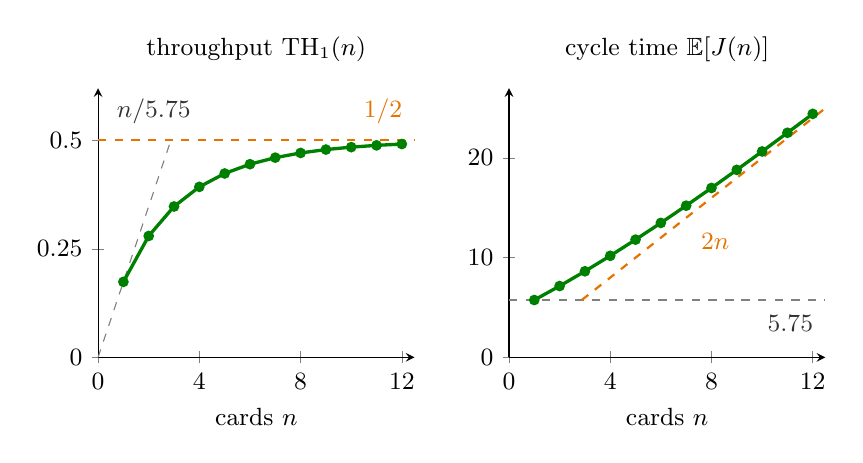
\begin{tikzpicture}[font=\small, >={Latex[length=2mm]}]
\begin{axis}[name=left, width=5.6cm, height=5.0cm, axis lines=left,
  xmin=0, xmax=12.5, ymin=0, ymax=0.62, xtick={0,4,8,12}, ytick={0,0.25,0.5},
  yticklabel style={/pgf/number format/fixed},
  xlabel={cards $n$}, title={throughput $\mathrm{TH}_1(n)$}, clip=false]
  \addplot[thin, gray, dashed, domain=0:2.875] {x/5.75};
  \addplot[thick, orange!90!black, dashed, domain=0:12.5] {0.5};
  \node[orange!90!black, anchor=south east] at (axis cs:12.4,0.515) {$1/2$};
  \node[gray!40!black, anchor=south] at (axis cs:2.2,0.515) {$n/5.75$};
  \addplot[very thick, green!50!black, mark=*, mark size=1.3pt] coordinates {(1,0.1739) (2,0.2796) (3,0.3475) (4,0.3927) (5,0.4235) (6,0.4449) (7,0.4600) (8,0.4708) (9,0.4786) (10,0.4842) (11,0.4883) (12,0.4913)};
\end{axis}
\begin{axis}[at={(left.east)}, anchor=west, xshift=1.2cm, width=5.6cm, height=5.0cm, axis lines=left,
  xmin=0, xmax=12.5, ymin=0, ymax=27, xtick={0,4,8,12}, ytick={0,10,20},
  xlabel={cards $n$}, title={cycle time $\mathbb{E}[J(n)]$}, clip=false]
  \addplot[thin, gray, dashed, domain=0:12.5] {5.75};
  \addplot[thick, orange!90!black, dashed, domain=2.875:12.5] {2*x};
  \node[gray!40!black, anchor=north east] at (axis cs:12.4,5.2) {$5.75$};
  \node[orange!90!black, anchor=north west] at (axis cs:7.2,13.4) {$2n$};
  \addplot[very thick, green!50!black, mark=*, mark size=1.3pt] coordinates {(1,5.750) (2,7.152) (3,8.633) (4,10.187) (5,11.807) (6,13.486) (7,15.216) (8,16.992) (9,18.806) (10,20.653) (11,22.527) (12,24.424)};
\end{axis}
\end{tikzpicture}
\end{document}
